%-------------------------
%minimal-unix
%(c) H.Buchmann FHNW 2017
%export TEXINPUTS=.:${HOME}/fhnw/edu/:${HOME}/fhnw/edu/tinL/config/latex:${HOME}/fhnw/edu/config//:
%-------------------------
\documentclass{beamer}
\usepackage{latex/beamer}
%---------------------
%local defines
%(c) H.Buchmann FHNW 2009
%$Id$
%---------------------
\newcommand{\target} {\beaglebone\xspace}
\newcommand{\targetS}{{\bf BBG}\xspace}
\newcommand{\host}   {{\em Host}\xspace}
\newcommand{\targetroot} {{\bf target-root}\xspace}
\newcommand{\kernel} {{\bf kernel}\xspace}
\renewcommand{\c}{{\bf C}\xspace}
\newcommand{\cpp}{{\bf C++}\xspace}
\newcommand{\posix}{{\bf POSIX}\xspace}


\usepackage[absolute]{textpos}
\setlength{\TPHorizModule}{1mm}
\setlength{\TPVertModule}{1mm}

\begin{document}

\newcommand{\md}{\cod{md-bbb-{\em version}.img}}
\newcommand{\mdev}{\cod{md-bbb-devel-{\em version}.tar.gz}}
\title[Minimal]{Ein kleines \unix}

\frame{\titlepage}

\begin{frame}{Ein kleines \unix}
 \begin{itemize}
  \item die einzelnen Komponenten
  \item für Test
  \item übersichtlich
  \item grosse Systeme haben ähnliche Komponenten
 \end{itemize}
\end{frame}

\begin{frame}{Die grossen Blöcke}{Übergänge}
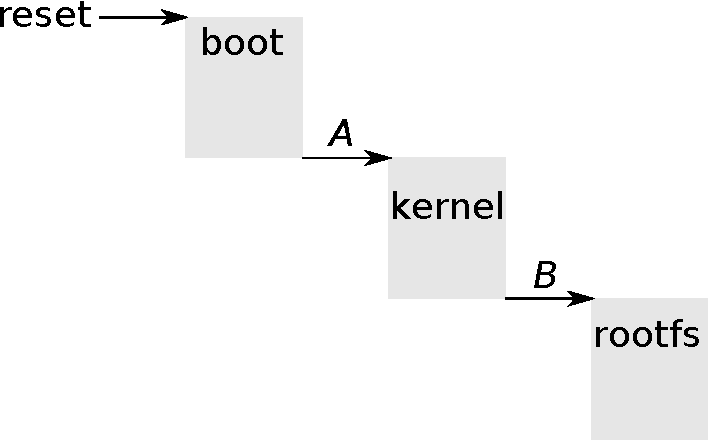
\includegraphics[width=\textwidth]{components.pdf}
\begin{textblock}{100}(10,50)
 \begin{description}[reset]
  \item[reset] start: BigBang
  \item[A] unprotected$\to$ protected ?
  \item[B] concurrency
 \end{description}
\end{textblock}
\end{frame}

\begin{frame}[fragile]{Boot:u-boot}{Zwei Files}
\begin{block}{reset}
{\tiny
\begin{verbatim}
U-Boot 2018.09 (Dec 18 2018 - 13:56:52 +0100)
\end{verbatim}
}
\end{block}
 \begin{itemize}
  \item \cod{MLO} Wegen TI
  \item \cod{u-boot.img}
 \end{itemize}
\begin{textblock}{100}(45,30)
 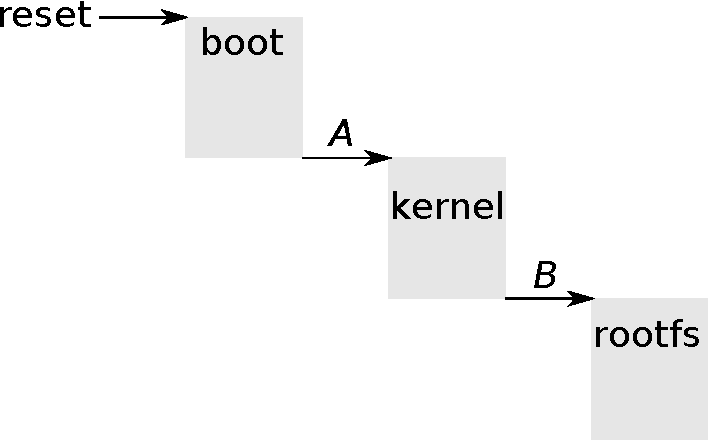
\includegraphics[width=0.75\textwidth]{components.pdf}
\end{textblock} 
\end{frame}

\begin{frame}[fragile]{Kernel}{Zwei Files}
\begin{block}{A}
{
\tiny
\begin{verbatim}
Booting Linux on physical CPU 0x0					       
Linux version 4.19.5 (buchmann@buchmannh) (gcc version 8.2.0 (GCC)) #6 SMP PRE8
\end{verbatim}
}
\end{block}
\begin{itemize}
 \item \cod{zImage} Der {\em kernel}
 \item \cod{am335x-boneblack-wireless.dtb} device tree
 \end{itemize}
\begin{textblock}{100}(45,30)
 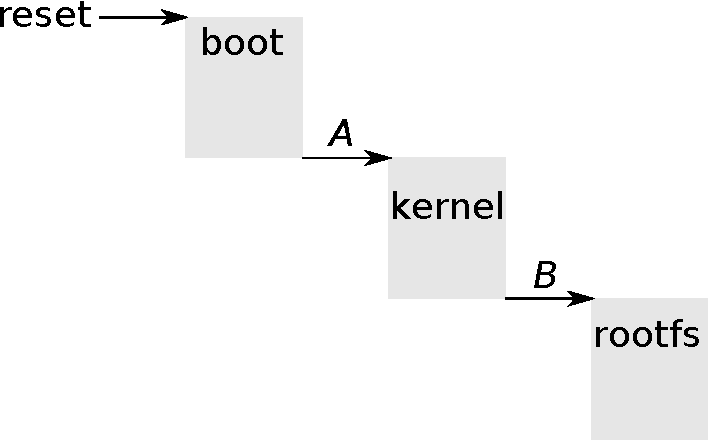
\includegraphics[width=0.75\textwidth]{components.pdf}
\end{textblock} 
\end{frame}

\begin{frame}[fragile]{RootFS: Viele Files}{Unser Interesse}
\begin{block}{B}
{
\tiny
\begin{verbatim}
VFS: Mounted root (ext4 filesystem) on device 179:2.
devtmpfs: mounted
Freeing unused kernel memory: 1024K

Please press Enter to activate this console. 
\end{verbatim}
}
\end{block}
\begin{itemize}
 \item \cod{linuxrc} Init-Process
 \item ...
\end{itemize}
\begin{textblock}{100}(45,25)
 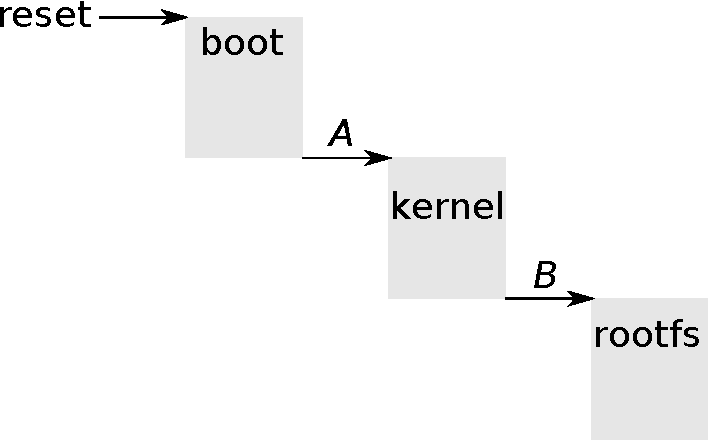
\includegraphics[width=0.75\textwidth]{components.pdf}
\end{textblock} 

\end{frame}

\begin{frame}{RootFS}{Flavours}
 \begin{itemize}
  \item nano
  \begin{itemize}
   \item Assembler ohne {\em libraries} \cod{s-nano.S}
   \item \c fast ohne {\em libraries} \cod{c-nano.c}
  \end{itemize}
  \item mini
  \begin{itemize}
   \item {\em libraries}
   \begin{itemize}
    \item static
    \item dynamic
   \end{itemize}
  \end{itemize}
  \item full
  \begin{itemize}
   \item \cod{busybox}
   \item \cod{ssh}
   \item ...
  \end{itemize}
 \end{itemize}
\end{frame}

\section{Nano}
\begin{frame}
\begin{center}
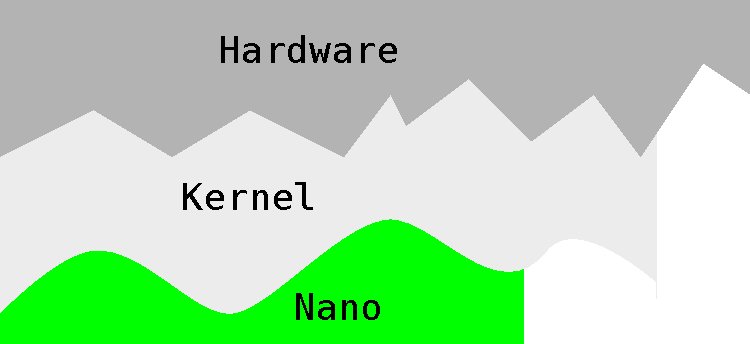
\includegraphics[width=0.75\textwidth]{nano.pdf}
\end{center}
\begin{itemize}
 \item \cod{config/Makefile}
 \item \cod{src/s-nano.S}
 \item \cod{src/c-nano.c}
\end{itemize}
\end{frame}

\section{Mini}
\begin{frame}
\begin{center}
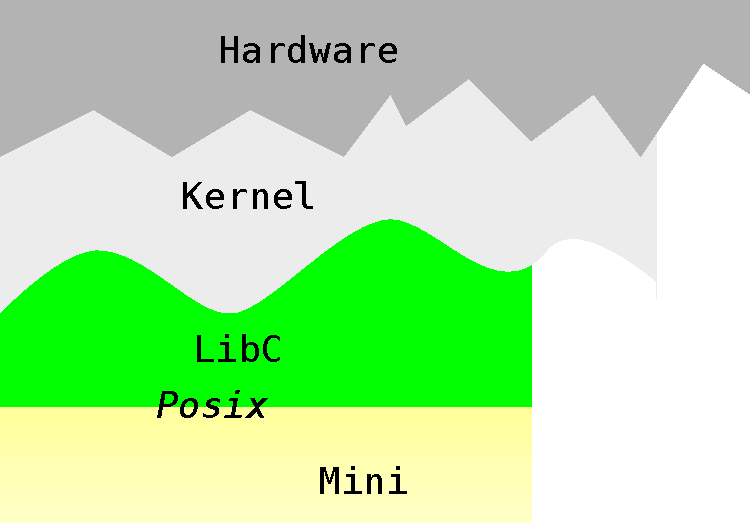
\includegraphics[width=0.75\textwidth]{mini.pdf}
\end{center}
\vspace{-5mm}
\begin{itemize}
 \item \cod{config/Makefile}
 \item \cod{src/mini.c}
 \begin{itemize}
  \item static
  \item dynamic
 \end{itemize}
\end{itemize}
\end{frame}

\subsection{Libraries}

\begin{frame}{Statische/Dynamische Bibliothek}{Kopie vs. Referenz}
 \begin{columns}
  \begin{column}{5cm}
   \begin{block}{Static}
   \begin{itemize}
    \item \hfill \vspace{-3mm}\fig{static.pdf}{0.5}{0}
    \item {\Large fr�hes} Binden
   \end{itemize}
   \end{block}
  \end{column}
  \begin{column}{5cm}
   \begin{block}{Dynamic}
    \begin{itemize}
    \item\hfill \vspace{-3mm}\fig{dynamic.pdf}{0.5}{0}
    \item {\Large sp�tes} Binden
    \end{itemize}
   \end{block}
  \end{column}
 \end{columns}
 \begin{block}{}
  \fig{legend.pdf}{0.5}{0}
 \end{block}
\end{frame}



\section{Aufgaben}

\begin{frame}{Ziel}
 \begin{itemize}
  \item \cod{hello-world} auf dem \host und auf dem \targetS
  \item \cod{primes} auf dem \host und auf dem \targetS
 \end{itemize}
\end{frame}


\begin{frame}{The big Picture}
 \begin{itemize}
  \item Source File: \cod{hello-world.cc}
  \item falls es nicht klapt ?
  \begin{itemize}
   \item wo ist der File ?
  \end{itemize}
 \end{itemize}
\end{frame}


%\subsection{Die Programme}
%\begin{frame}{Development}{\cod{hello-world-c.c}}
%\hspace*{-8mm}
%{
%\begin{tabular}{llllll}
% Host & Target & OS & Toolchain & Verbindung & Bemerkungen\\
% \hline
% \targetS & \targetS & Debian & mitgeliefert&&\\
% \host   & \targetS & Debian & \cod{\tiny tc-tinl-gcc-8.1.0-2018.05.21.tar.gz} & sshfs\\
% \host   & \targetS & minimal & \cod{\tiny tc-tinl-gcc-8.1.0-2018.05.21.tar.gz} & SD-Card  &später\\
% \host   & \targetS & minimal & \cod{\tiny tc-tinl-gcc-8.1.0-2018.05.21.tar.gz} & curlftpfs&später\\
%\end{tabular}
%}
%\remark{Toolchain auf der Cloud: \href{https://drive.switch.ch/index.php/s/A6H382zEGDrgfAL}
%       {\Huge tinL}}
%\end{frame}

%-------------------------
%minimal-unix
%(c) H.Buchmann FHNW 2017
%export TEXINPUTS=.:${HOME}/fhnw/edu/:${HOME}/fhnw/edu/tinL/config/latex:${HOME}/fhnw/edu/config//:
%-------------------------
\documentclass{beamer}
\usepackage{latex/beamer}
%---------------------
%local defines
%(c) H.Buchmann FHNW 2009
%$Id$
%---------------------
\newcommand{\target} {\beaglebone\xspace}
\newcommand{\targetS}{{\bf BBG}\xspace}
\newcommand{\host}   {{\em Host}\xspace}
\newcommand{\targetroot} {{\bf target-root}\xspace}
\newcommand{\kernel} {{\bf kernel}\xspace}
\renewcommand{\c}{{\bf C}\xspace}
\newcommand{\cpp}{{\bf C++}\xspace}
\newcommand{\posix}{{\bf POSIX}\xspace}


\usepackage[absolute]{textpos}
\setlength{\TPHorizModule}{1mm}
\setlength{\TPVertModule}{1mm}

\begin{document}
\title{Minimaler target-root}
\frame{\titlepage}

\begin{frame}{Ziel}
 \begin{itemize}
  \item Zwei \cod{target-root}'s
  \begin{itemize}
   \item für {\em development} auf dem \host für \targetS
   \item für {\em runtime} auf dem \targetS
  \end{itemize}
 \end{itemize}
\end{frame}

\begin{frame}{Zwei \cod{target-root}'s}{identisch}
\begin{minipage}{0.375\textwidth}
{
\dirtree{%
.0 \host.
.1 lib.
.1 usr.
.2 include.
.2 lib.
}
}
\end{minipage}
\begin{minipage}{0.375\textwidth}
{
\dirtree{%
.0 \targetS
.1 lib.
.1 usr.
.2 include.
.2 lib.
}
}
\end{minipage}
\end{frame}


\begin{frame}{Typische Beispiele}
 \begin{itemize}
  \item C
  \begin{itemize}
   \item \cod{c-hello.c} einfaches Programm
  \end{itemize}
  \item C++
  \begin{itemize}
   \item \cod{cc-hello.cc} einfaches Programm
   \item \cod{cc-threads.cc} komplexes Programm
  \end{itemize}
 \end{itemize}
\end{frame}

\subsection{\cod{c-hello.c}}
\begin{frame}{Development}{\target}
 \begin{itemize}
  \item compile
  \begin{itemize}
   \item source files
   \item include files
  \end{itemize}
  \item link
  \begin{itemize}
   \item object Files \cod{*.o}
   \item static libraries \cod{*.a}
  \end{itemize}
 \end{itemize}
\end{frame}

\begin{frame}{Execution}
 \begin{itemize}
  \item dynamic libraries \cod{*.so}
  \item executables
 \end{itemize}
\end{frame}

\begin{frame}{Aufteilung}
 \begin{itemize}
  \item source/include Files $to$ \host
  \item \cod{*.o} \cod{*.a} $to$ \host
  \item dynamic libraries \cod{*.so} $to$ \targetS
  \item executables $to$ \targetS 
 \end{itemize}
\end{frame}

\begin{frame}{Aufgaben}
 \begin{itemize}
  \item Aufteilung für \cod{c-hello}
  \item Aufteilung für \cod{cc-hello}
  \item Aufteilung für \cod{cc-threads}
 \end{itemize}
 \begin{itemize}
  \item Füjhren Sie Buch über die Aufteilung:
  \begin{itemize}
   \item die Grösse der beiden Verzeichnisse
   \item die Anzahl Files in beiden Verzeichnisse
  \end{itemize}
 \end{itemize}
\end{frame}
\end{document}

\end{document}
